\newpage
\section{Least squares fitting and interpolation}
Given data represented by a set of points $[(x_i, y_i)]$, where $x_i$ is the control variable and $y_i$ is the observable (e.g., I control the current through a resistor and observe the voltage), the least-squares fit to a function $f(x; p_1, p_2, ... p_n)$ minimizes the sum of squared residuals, i.e.,
\begin{equation}
    R^2 = \sum_i \left|f(x_i, \{p\}) - y_i\right|^2.
\end{equation}
The result of the fit is a set of parameters $p_1, p_2, p_3, ...$ which minimize $R^2$. Depending on how the function $f$ depends on the parameters $p_k$ we talk about \emph{linear} or \emph{non-linear} fitting. The important difference is the dependence on the parameters $p$, not on the control variable $x$. 

% \subsection{Linear Regression}
% TODO

\subsection{Polynomial fitting.}
Fitting a polynomial in $x$ where the fit parameters are the coefficients of the polynomial is a very common example of linear fitting. Interface for using polynomials is contained in \ls{np.polynomial} submodule in the \ls{Polynomial} class, which provides a 

\lstinputlisting[caption=Polynomial fitting]{../example_code/polynomial_fitting_example.py}
\begin{center}
    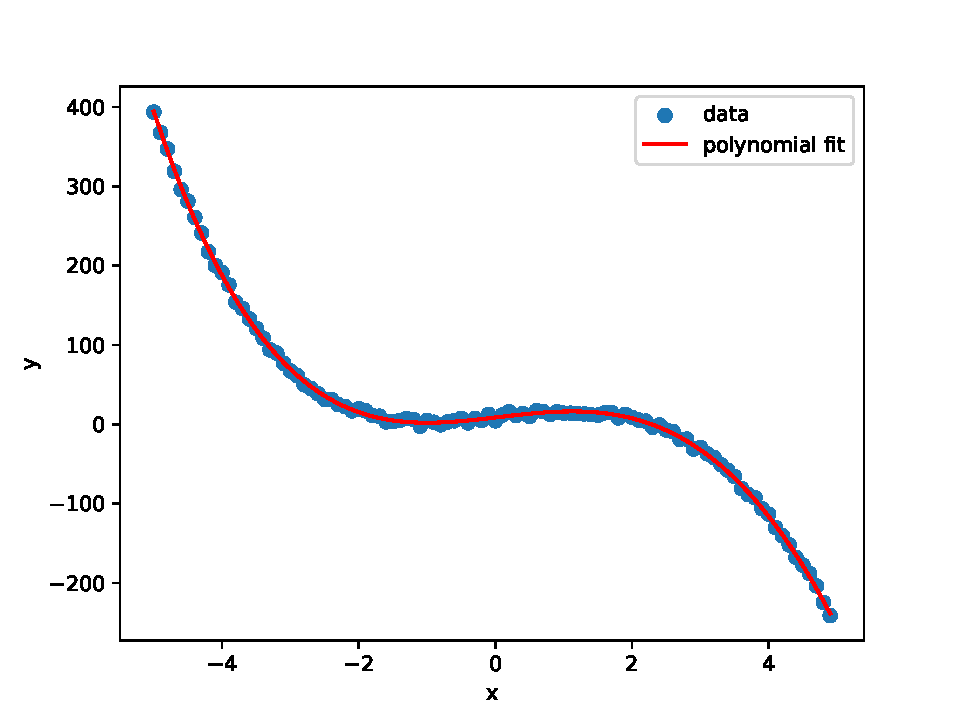
\includegraphics[width=0.5\linewidth]{polynomial_fit.pdf}
\end{center}

\begin{exercise}
    Remove the background from the peaks in exercise~\ref{ex:peaks} using a polynomial fit.

    \emph{Hint}: \ls{np.polynomial.Polynomial.fit()} and boolean arrays
\end{exercise}

\subsection{Non-linear curve fitting}
When the fitting function depends nonlinearly on the fit parameters we need to use nonlinear fitting, several libraries exist for this task, and for basic fitting, we can use \ls{scipy.optimize} submodule of \ls{scipy}.

To fit a given function to data we can use \ls{scipy.optimize.curve_fit}, e.g.,
\lstinputlisting[caption=Nonlinear curve fitting., label=lst:curve-fit]{../example_code/curve_fit_example.py}
\begin{center}
    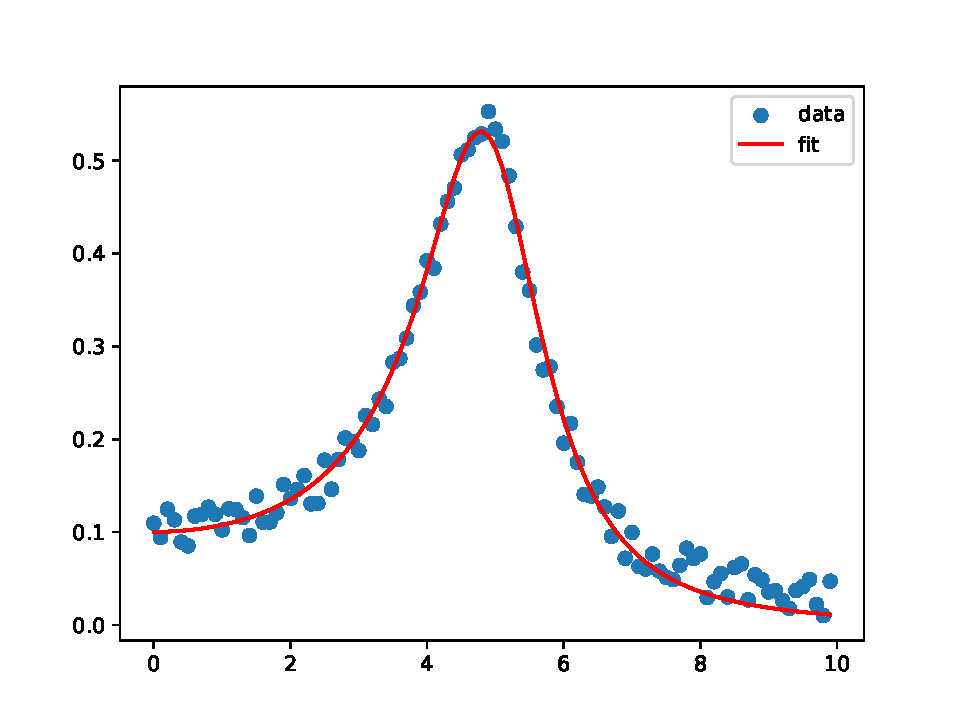
\includegraphics[width=0.5\linewidth]{curve_fit.pdf}
\end{center}

Unlike linear least squares, non-linear curve fitting is iterative and stops once the parameters converge. The fit may never converge for certain problems, therefore, once a configured maximum number of iterations is exceeded the fitting routines \emph{raise an exception} (See \ref{syn:exceptions}) which will crash the program if not handled.

We can use \ls{scipy.optimize.minimize()} for more general optimisation problems. \ls{minimize()} takes a single \textbf{scalar} function and an initial guess for the optimal parameters. For example, to find a minimum of a parabola,
\lstinputlisting[caption=Minimization of a scalar function of multiple parameters.]{../example_code/minimize.py}
\begin{center}
    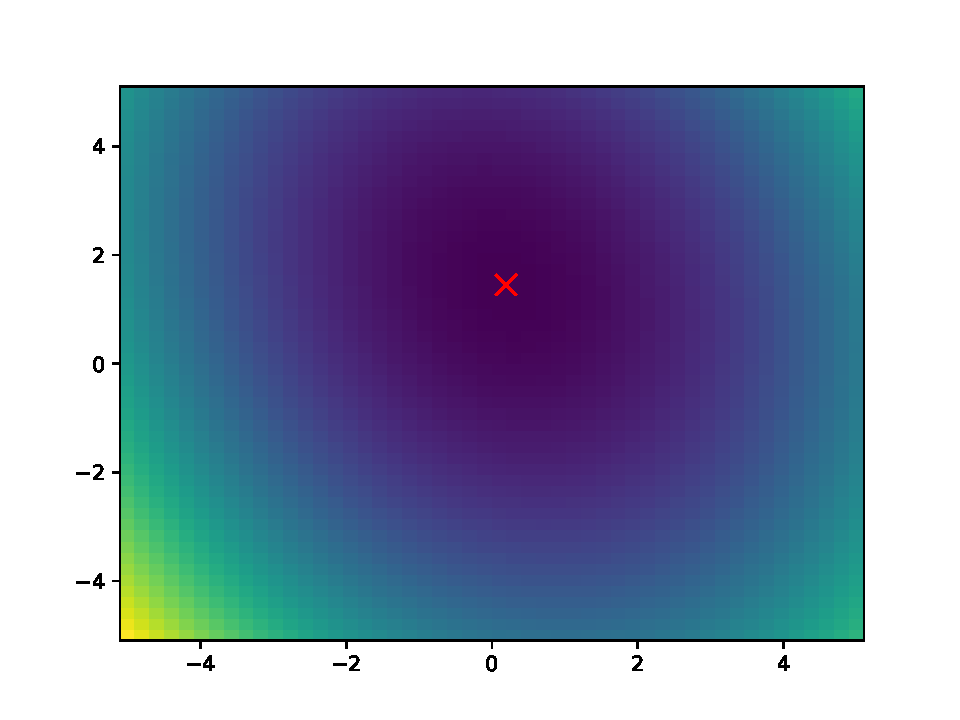
\includegraphics[width=0.5\linewidth]{parabola-minimize.pdf}
\end{center}

\paragraph{Parameter error estimation} The fitting function \ls{curve_fit} returns two values -- the array of the parameters we are interested in and the covariance matrix of the parameters, i.e., $\mathrm{cov}(p_i, p_j) = \langle(p_i - \bar p_i)(p_j - \bar p_j)\rangle$. The diagonal values of the covariance matrix can be used as an estimate of the uncertainties of the fit parameters, i.e.,
\begin{lstlisting}
    #assuming that f is def'ed as f(x, p1, p2)
    p, cov = curve_fit(f, x, y)
    print(f"p1 = {p[0]} +/- {np.sqrt(cov[0,0])}
\end{lstlisting}

The covariance matrix is calculated from the \textit{residuals} $r_i = y_i - f(x_i, \{p_j\})$, where $p_j$ are the optimized parameters as ($\mathbf{r}$ is a vector with elements $r_i$; $i=1\dots N$, $j=1\dots M$) as a scaled inverse of the Hessian matrix $H$ of the objective function $\chi^2 = \sum r_i^2$\footnote{The calculation is slightly more complicated, but similar, when the data points have different weights, see documentation \url{https://docs.scipy.org/doc/scipy/reference/generated/scipy.optimize.curve_fit.html}}
\begin{equation}
    \mathrm{cov}(p_i, p_j) = \frac{1}{N-M}
    \begin{pmatrix}
        \frac{\partial \chi^2}{\partial p_1 \partial p_1} & \frac{\partial \chi^2}{\partial p_1 \partial p_2} & \dots \\
        \frac{\partial \chi^2}{\partial p_1 \partial p_1} & \frac{\partial \chi^2}{\partial p_2 \partial p_2} & \dots\\
        \vdots & \vdots & \ddots
    \end{pmatrix}^{-1},
\end{equation}
where $N$ is the number of data points and $M$ is the number of parameters. Note that usually, we are interested only in the diagonal for the direct error estimate of the fit parameters, however, if, for example, the studied quantity is a sum of two fit parameters $z = A + B$, then the variance of $z$
\begin{equation}
    \mathrm{var} z = \langle (A + B - \bar A - \bar B)^2 \rangle = \langle (A - \bar A)^2 \rangle + \langle (B - \bar B)^2 \rangle + 2\langle (A - \bar A) (B - \bar B) \rangle = \mathrm{var} A + \mathrm{var} B + 2\mathrm{cov}(A, B),
\end{equation}
and the off-diagonal terms of the covariance matrix must be used.

However, the error estimates calculated using the covariance matrix can often be underestimated since the above method is valid only when the model function $f$ is correct and the data truly have the form $y_i = f(x_i, p) + e_i$ where data errors $e_i$ have zero mean and a normal distribution. A more robust, but also more computationally demanding, method of estimating parameter errors is \textbf{bootstrap}, where, for several repetitions, we create a random selection of data (of the same length), perform the fit on each created set and calculate mean and standard deviation (and in principle covariance) on the resulting set of fit parameters, an example implementation is shown in Lst.~\ref{lst:bootstrap}

\lstinputlisting[firstline=24, caption=Estimating fit parameter errors using bootstrap. The data $(x_i\, y_i)$ are created in the same way as in Lst.~\ref{lst:curve-fit}., label=lst:bootstrap]{../example_code/bootstrap_curve_fit_example.py}

\begin{syntax}[Exceptions and error handling]
    \label{syn:exceptions}
    Exceptions are a mechanism used by Python to signal errors or other events which need to be handled by your code. If a \emph{raised} exception is not \emph{caught} the program crashes. To handle exceptions we use the \ls{try}, \ls{except}, and \ls{finally} blocks. We can raise an exception using \ls{raise}. Note that exceptions do not always have to indicate an error, for example, a \ls{for} loop is terminated using a \ls{StopIteration} exception.

    Example of catching and raising exceptions and using the \ls{finally} block.
\begin{lstlisting}

def faulty_function():
    raise ValueError("blergh!")

xs = [-2, -1, 0, 1, 2]
one_over_xs = []
try:
    for x in xs:
        try:
            one_over_xs.append(1/x)
            if x > 1:
                faulty_function()
        except ZeroDivisionError:
            print("Can't divide by zero!")
        except:
            print("something else went wrong")
            raise #propagate the exception further up
finally:
    print("I will always run")

# unless the exception that is raised on line 8 and then sent forward on line 13 isn't
# handled, this line will not run
print(one_over_xs)
\end{lstlisting}
    Notice a few things:
    
    \textbf{\ls{except}} Can catch either a specific type of exception or any type (if the exception type is not specified).
    
    \textbf{\ls{finally} block always runs}, regardless of whether an exception occurred inside the \ls{try} block and is generally meant for proper cleanup (e.g., open files)
        
    \textbf{\ls{try} blocks can be nested}: When an exception is raised, the inner-most \ls{try-except} block tries to handle it. If a suitable \ls{except} is not found or the exception is re-\ls{raise}d, the next enclosing \ls{try-except} block tries to handle it and so on. If the exception gets out of all nested enclosing \ls{try-except} blocks without being handled, the program crashes.
    
    \textbf{\ls{raise} can be used anywhere}, e.g., in functions which do not contain \ls{try}. It is up to the calling code to decide what to do with exceptions
\end{syntax}

\begin{exercise}
    \label{ex:peak-fits}
    Fit the absolute value $r(f) = \sqrt{x^2 + y^2}$ of the response in exercise~\ref{ex:peaks} to the response of a linear harmonic oscillator plus a polynomial background (polynomial degree 3) and plot the results similarly to exercise~\ref{ex:peaks}. Use the simple estimation from exercise~\ref{ex:peak} as initial estimates of the fit parameters. Use the solution to exercise~\ref{ex:peak} as a module.

    Bonus exercise: make the background polynomial degree adjustable

    The complex amplitude of the response of a linear harmonic oscillator to force $F$ is (see Appendix.~\ref{sec:lho})
    \begin{equation}
        x(\omega) = \frac{F/m}{\omega_0^2 - \omega^2 + i\omega\gamma},
    \end{equation}
    where $\omega_0$ is the (angular) resonance frequency, $\omega$ is the frequency of the force $F$, $m$ is the oscillator mass and $\gamma$ is damping.
\end{exercise}
\begin{exercise}
    Estimate the errors of fitting parameters obtained in exercise~\ref{ex:peak-fits} using bootstrap.
\end{exercise}

% lmfit